%%%%
%%%% Multiagent Simulation and the MASON Library
%%%% GeoMason GIS extension
%%%%
%%%% Copyright 2012 by Mark Coletti
%%%%
%%%% LaTeX Source
%%%% This source code, and embedded PDFs and sources (such as OmniGraffle Files)
%%%% Are distributed under the Academic Free License version 3.0
%%%% See the file "LICENSE" for more information
%%%%
%%%% When you build this source code, the resulting PDF file is licensed under the
%%%% Creative Commons Attribution-No Derivative Works 3.0 United States License
%%%% See the URL http://creativecommons.org/licenses/by-nd/3.0/us/   for more information
%%%%
%%%% If you have any questions, feel free to contact me at mcoletti@gmail.com

\documentclass[twoside,10pt]{book}
\usepackage{fullpage}
\usepackage{mathpazo}
\usepackage[noend]{algpseudocode}
\usepackage{amsmath}
\usepackage{latexsym}
\usepackage{graphicx}
\usepackage{wrapfig}
\usepackage{bm}
\usepackage{qtree}
\usepackage{array}
\usepackage{eurosym}
\usepackage{textcomp}
\usepackage{makeidx}
\usepackage{rotating}
\usepackage{multirow}
\usepackage{multicol}
\usepackage{microtype}
\usepackage{afterpage}
\usepackage{color}\definecolor{gray}{gray}{0.5}
\usepackage{xcolor}
\usepackage{alltt}
\usepackage{fancyvrb}
\usepackage[font=footnotesize,labelsep=quad,labelfont=it]{caption}
%%% Added in order to use hyperref -- this stuff has to appear before bibentry,x
%%% which has a conflict with regard to \bibitem.  See later in this file for more stuff that has
%%% to be added afterwards
  \makeatletter
  \let\saved@bibitem\@bibitem
  \makeatother

\usepackage{bibentry}
\usepackage[hyperfootnotes=false,linktocpage=true,linkbordercolor={0.5 0 0}]{hyperref}
%%% Note that to avoid a link being created from \pageref, just use \pageref*
%%% End hyperref stuff

\renewcommand\textfraction{0.0}
\renewcommand\topfraction{1.0}
\renewcommand\bottomfraction{1.0}


\newcommand\file[1]{\textsf{#1}}
\newcommand\variable[1]{\textsf{#1}}
%\newcommand\package[1]{\textsf{#1}}
\newcommand\package[1]{\index{Packages!{#1}}\textsf{#1}}
\newcommand\Package[1]{\index{Packages!{#1}|textbf}\textsf{#1}}
%\newcommand\class[1]{\textsf{#1}}
\newcommand\class[1]{\index{Classes!{#1}}\textsf{#1}}
\newcommand\Class[1]{\index{Classes!{#1}|textbf}\textsf{#1}}
\newcommand\method[1]{\textsf{#1}}
\newcommand\parameter[1]{\texttt{#1}}
\newcommand\character[1]{\texttt{"{#1}"}}
\newcommand\textstr[1]{\texttt{"{#1}"}}
\newcommand\code[1]{\textsf{#1}}
%\newcommand\code[1]{\texttt{#1}}

\newcommand\ignore[1]{}


\newcommand\sidebara[3]{\begin{wrapfigure}{r}[0in]{3.2in}%
\vspace{-1.1em}\hfill\framebox{\begin{minipage}{3in}\setlength\parindent{1.5em}\footnotesize{\noindent\textit{#1}

\vspace{0.5em}{\noindent #2}}
\end{minipage}}
\vspace{#3}
\end{wrapfigure}
}

\newcommand\sidebar[2]{\begin{wrapfigure}{r}[0in]{3.2in}%
\vspace{-1.1em}\hfill\framebox{\begin{minipage}{3in}\setlength\parindent{1.5em}\footnotesize{\noindent\textit{#1}

\vspace{0.5em}{\noindent #2}}
\end{minipage}}
\vspace{-0.5em}
\end{wrapfigure}
}



%%% Hack to allow more spacing before and after an hline
\newcommand\tstrut{\rule{0pt}{2.4ex}}
\newcommand\bstrut{\rule[-1.0ex]{0pt}{0pt}}

% Increase the numbering depth
\setcounter{secnumdepth}{3}
\setcounter{tocdepth}{6}


%%%% This code is used to create consistent lists of methods

% From TUGboat, Volume 24 (2003), No. 2 "Hints & Tricks"
\newcommand*{\xfill}[1][0pt]{%
	\cleaders
		\hbox to 1pt{\hss
			\raisebox{#1}{\rule{1.2pt}{0.4pt}}%
			\hss}\hfill}
			
\newenvironment{methods}[1]{
\vspace{1.0em}\noindent\textsf{\textbf{#1 Methods}}\quad \xfill[0.5ex]
\vspace{-0.25em}
\begin{description}
\small}
{\end{description}\hrule\vspace{1.5em}}

\newcommand{\mthd}[1]{\item[{\sf #1}]~\newline}


\newcommand\reference[1]{\vspace{0.5em}\hfill{\parbox{6in}{\raggedleft\noindent\textsf{#1}}}}

% Include subsubsection in the TOC
\setcounter{tocdepth}{3}

% Use with a %, like this:   \params{%
\newcommand\params[1]{\vbox{\begin{quote}\small\tt{\noindent{#1}}\end{quote}}}
\newcommand\script[1]{\params{#1}}
\newcommand\java[1]{\params{#1}}

% Allow poor horizontal spacing
\sloppy

% Allow a ragged bottom even in two-sided
\raggedbottom

% Command to push text to following page without the cutoff that occurs with clearpage
\newcommand\bump{\vspace{10in}}

% Command to push text to following line
\newcommand\hbump{\hspace{10in}}


% Define an existing word in text as an index item
\newcommand{\idx}[1]{\index{#1}#1}

% Define an existing word in text as an index item and make it bold
\newcommand{\df}[1]{\index{#1}\textbf{#1}}

% Provide a separate index item for a word in text and make it bold
\newcommand{\dfa}[2]{\index{#1}\textbf{#2}}

% Create algorithms and definitions
\newtheorem{algm}{Algorithm}
\newtheorem{defn}{Definition}

% Initial figures, pages, algorithms, and sections should be 0 :-)
\setcounter{figure}{-1}	% Mona is Figure 0
\setcounter{page}{-1}	% Start with Page 1 (the Front Page).  I'd like it to be Page 0 but it messes up twosided
\setcounter{algm}{-1}	% Start with Algorithm 0 (the Example Algorithm)
\setcounter{section}{-1}	% Start at Section 0 (the Introduction)

\thispagestyle{plain}
\thispagestyle{empty}

\newcommand\hsp[1]{{\rule{0pt}{0pt}\hspace{#1}}}
\newcommand\spc{{\rule{0pt}{0pt}~}}



\makeindex


\begin{document}

\begin{wrapfigure}{r}[2.5in]{4in}
\vspace{-1.1in}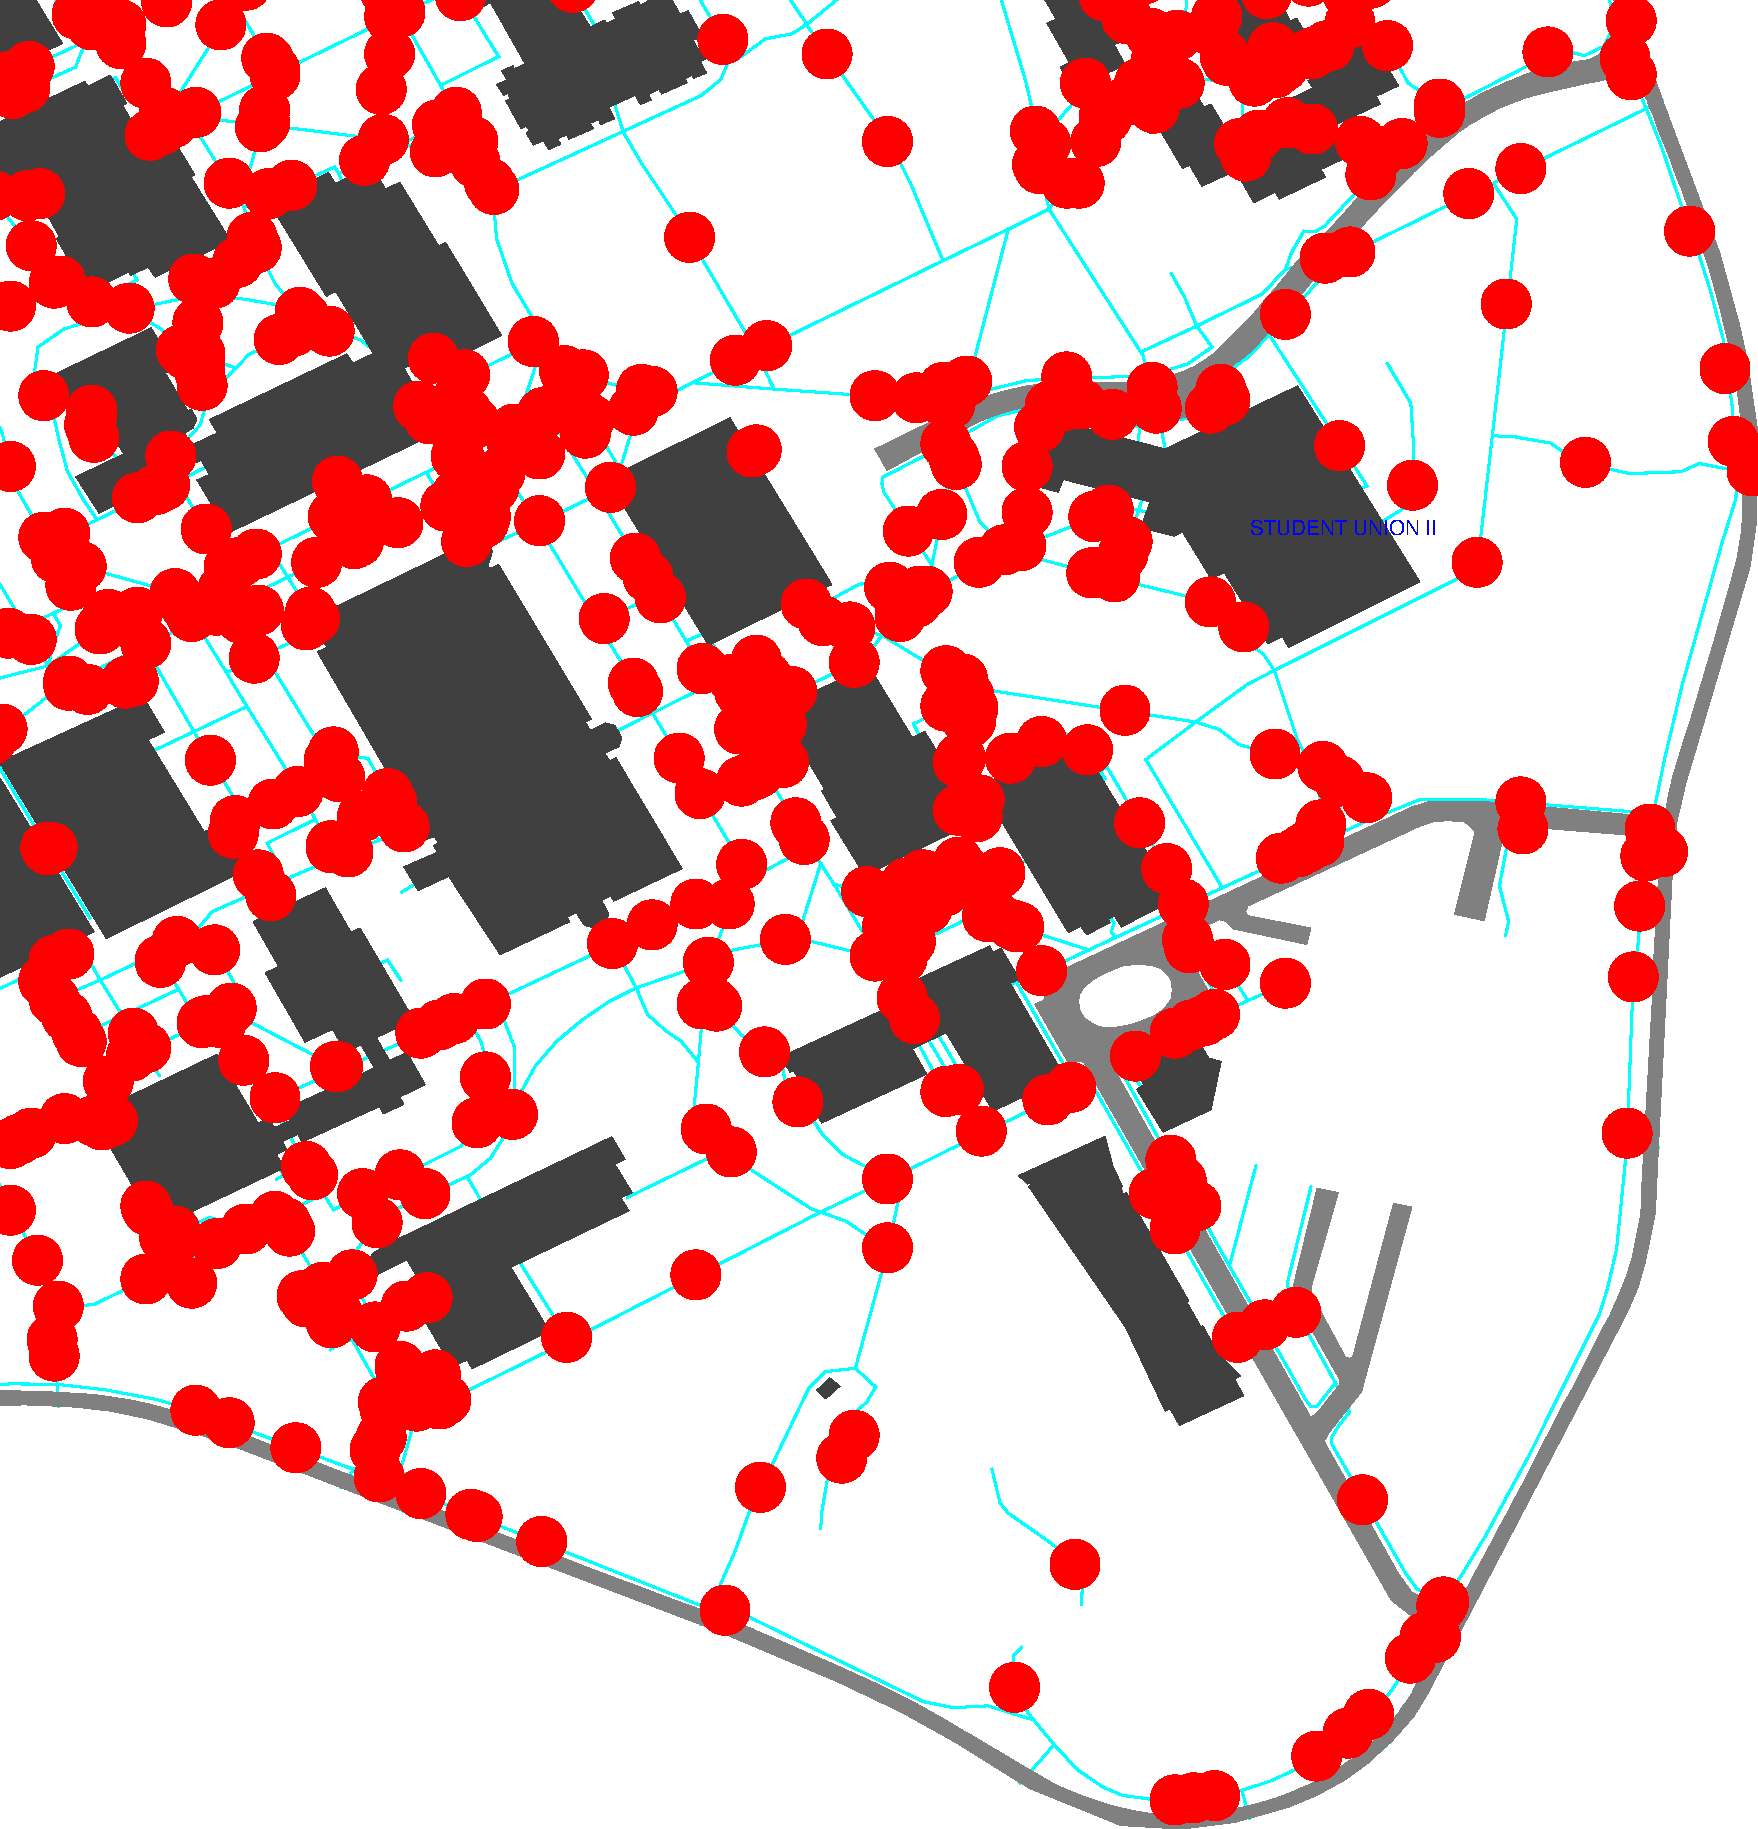
\includegraphics[height=11in]{campus.pdf}
\end{wrapfigure}

\begin{flushleft}
\huge\bf The GeoMason Cookbook\\[\baselineskip]
\end{flushleft}

\noindent\Large\bf Mark Coletti\\
{\large\rm 
Department of Computer Science\\
George Mason University}
\\
\\
\\
\Large\bf Zeroth Edition\\
\large\rm Online Version 0.0\\
\large\rm September, 2012\\

\vspace{5in}
\noindent\Large\bf Where to Obtain GeoMason\\
\large\rm http:/\!/cs.gmu.edu/\!\(\sim\)eclab/projects/mason/extensions/geomason/

\clearpage

\small 
\noindent {\Large\bf Copyright }  2012 by Mark Coletti.

\vspace{0.25in}
\noindent {\Large\bf Thanks to } Sean Luke, Andrew Crooks, Keith Sullivan

\vspace{0.25in}

\noindent {\Large\bf Get the latest version of this document or suggest improvements here:}

\reference{http:/\!/cs.gmu.edu/\!\(\sim\)eclab/projects/mason/extensions/geomason}

\vspace{0.15in}

\vspace{0.15in}
	\noindent {\Large\bf This document is licensed} under the {\bf Creative Commons Attribution-No Derivative Works 3.0 United States License,} except for those portions of the work licensed differently as described in the next section. To view a copy of this license, visit http:/\!/creativecommons.org/licenses/by-nd/3.0/us/ or send a letter to Creative Commons, 171 Second Street, Suite 300, San Francisco, California, 94105, USA.  A quick license summary:
	\begin{itemize}
	\item You are free to redistribute this document.
	\vspace{-0.5em}\item {\bf You may not} modify, transform, translate, or build upon the document except for personal use.   
	\vspace{-0.5em}\item You must maintain the author's attribution with the document at all times.
	\vspace{-0.5em}\item You may not use the attribution to imply that the author endorses you or your document use.  
	\end{itemize}
	This summary is just informational: if there is any conflict in interpretation between the summary and the actual license, the actual license always takes precedence.


\normalsize
\cleardoublepage

\tableofcontents
\clearpage


\chapter{Introduction}
\label{ch:intro}

\begin{figure}[h]\vspace{-33em}\hspace{30em}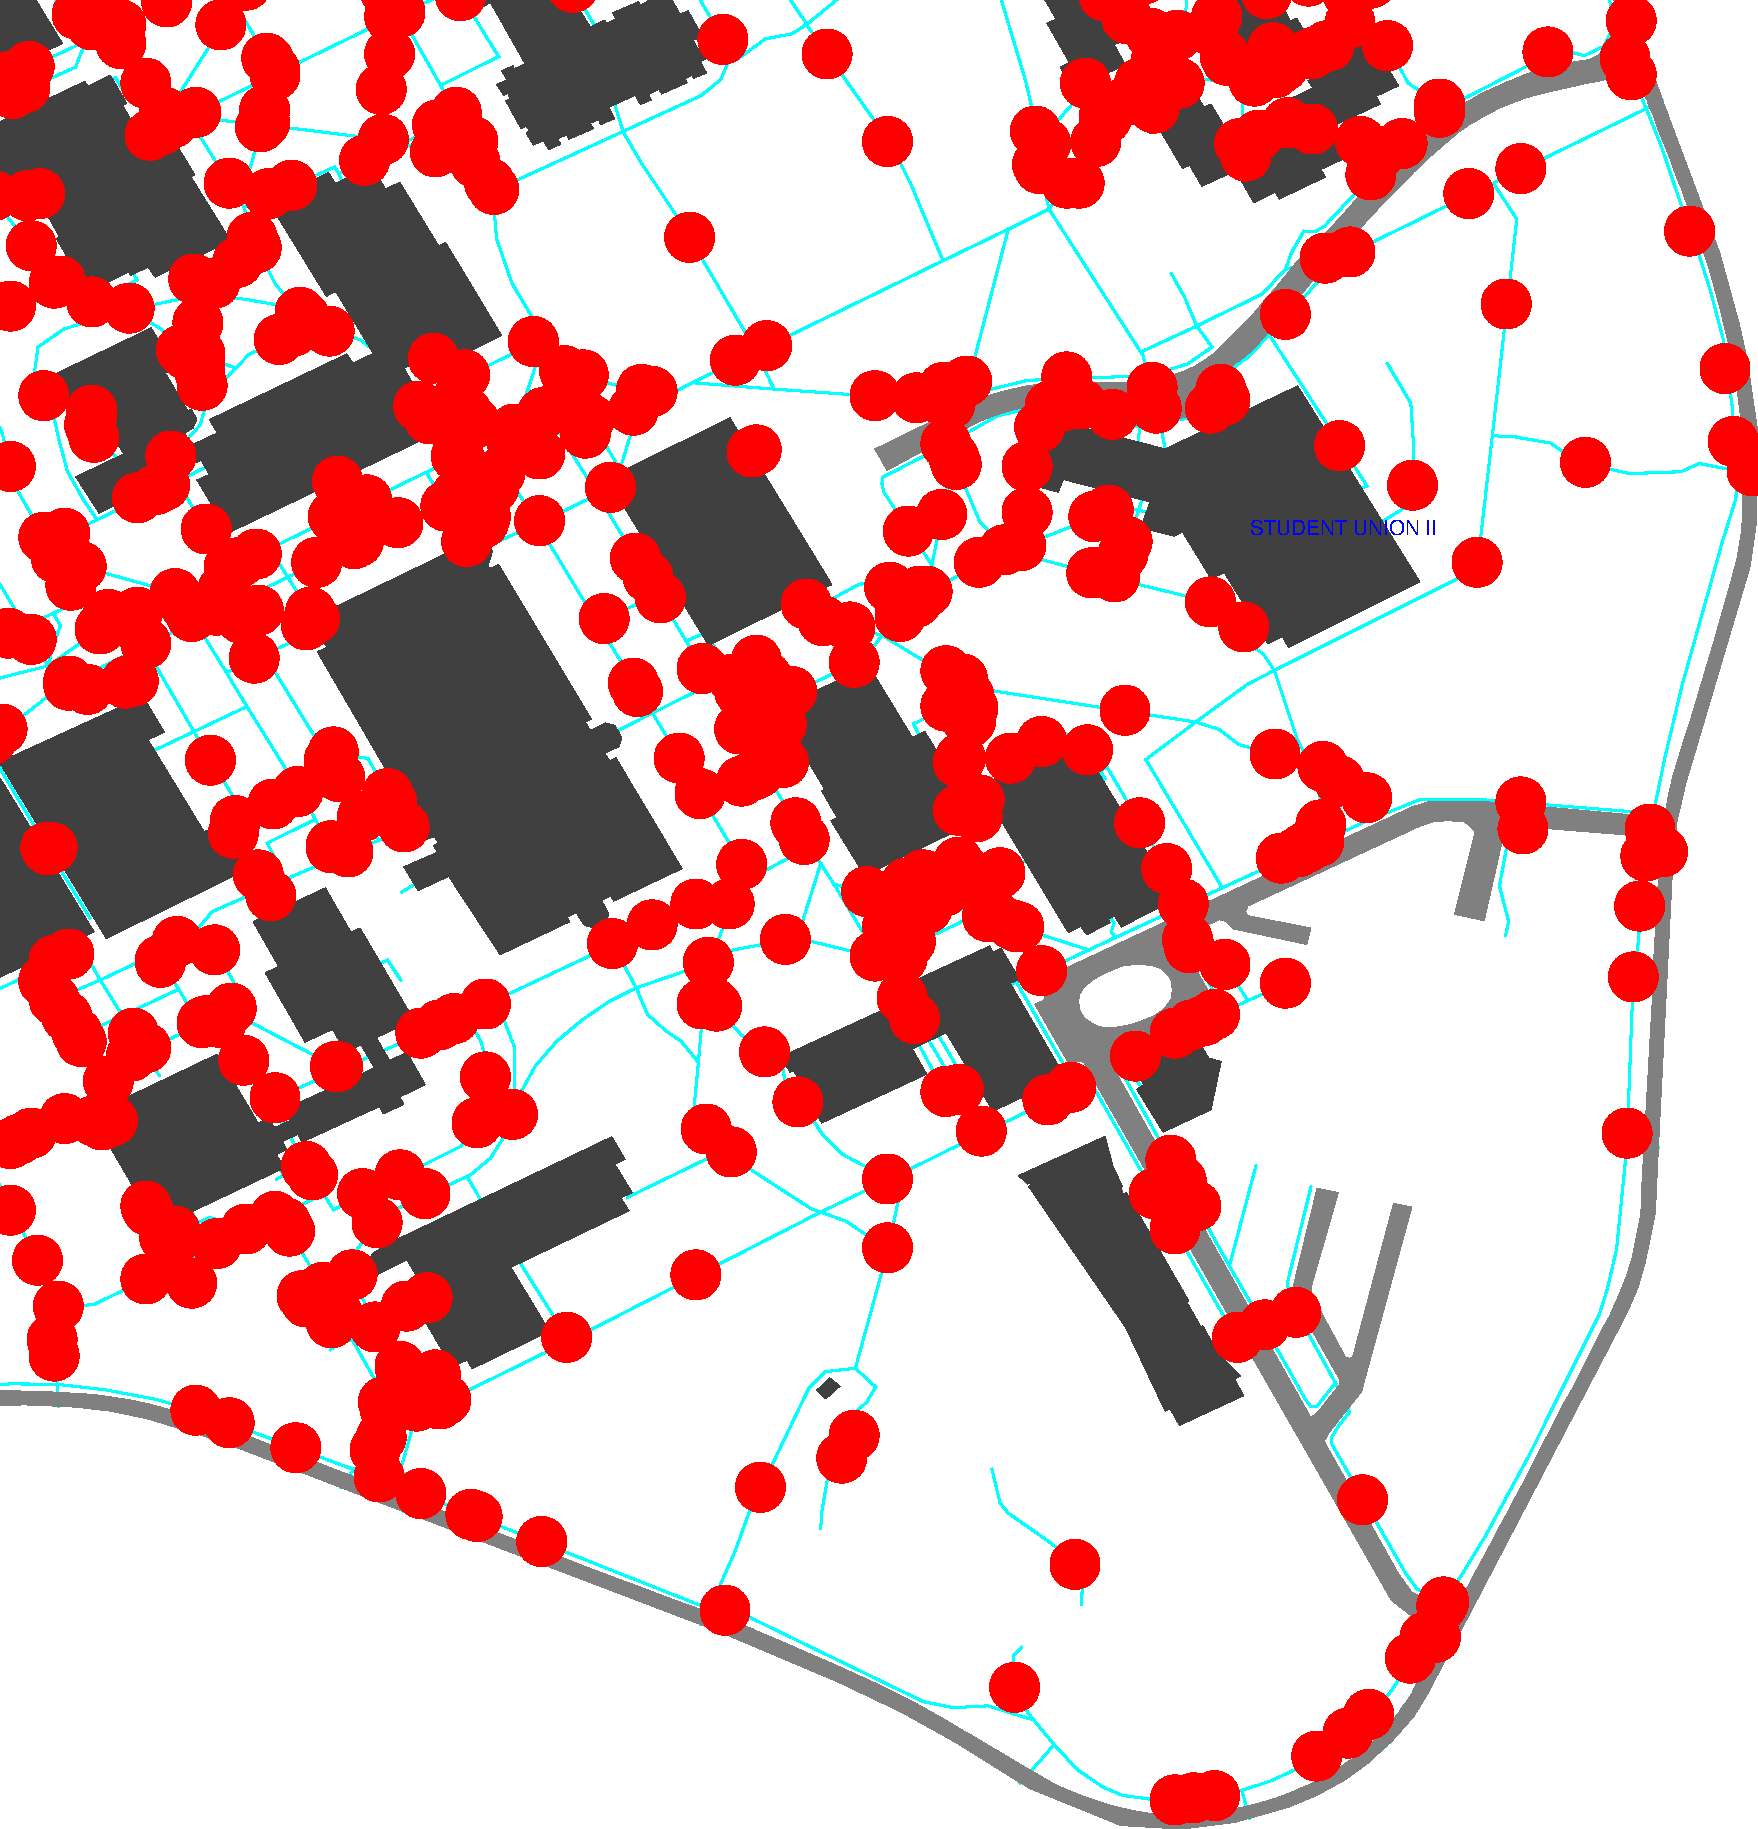
\includegraphics[width=4in]{campus.pdf}\vspace{2em}\end{figure}

GeoMason is a MASON extension that adds basic geospatial capability.

\section{Architectural Layout}

%\begin{wrapfigure}{r}[0in]{3.7in}
%\vspace{-4em}\hfill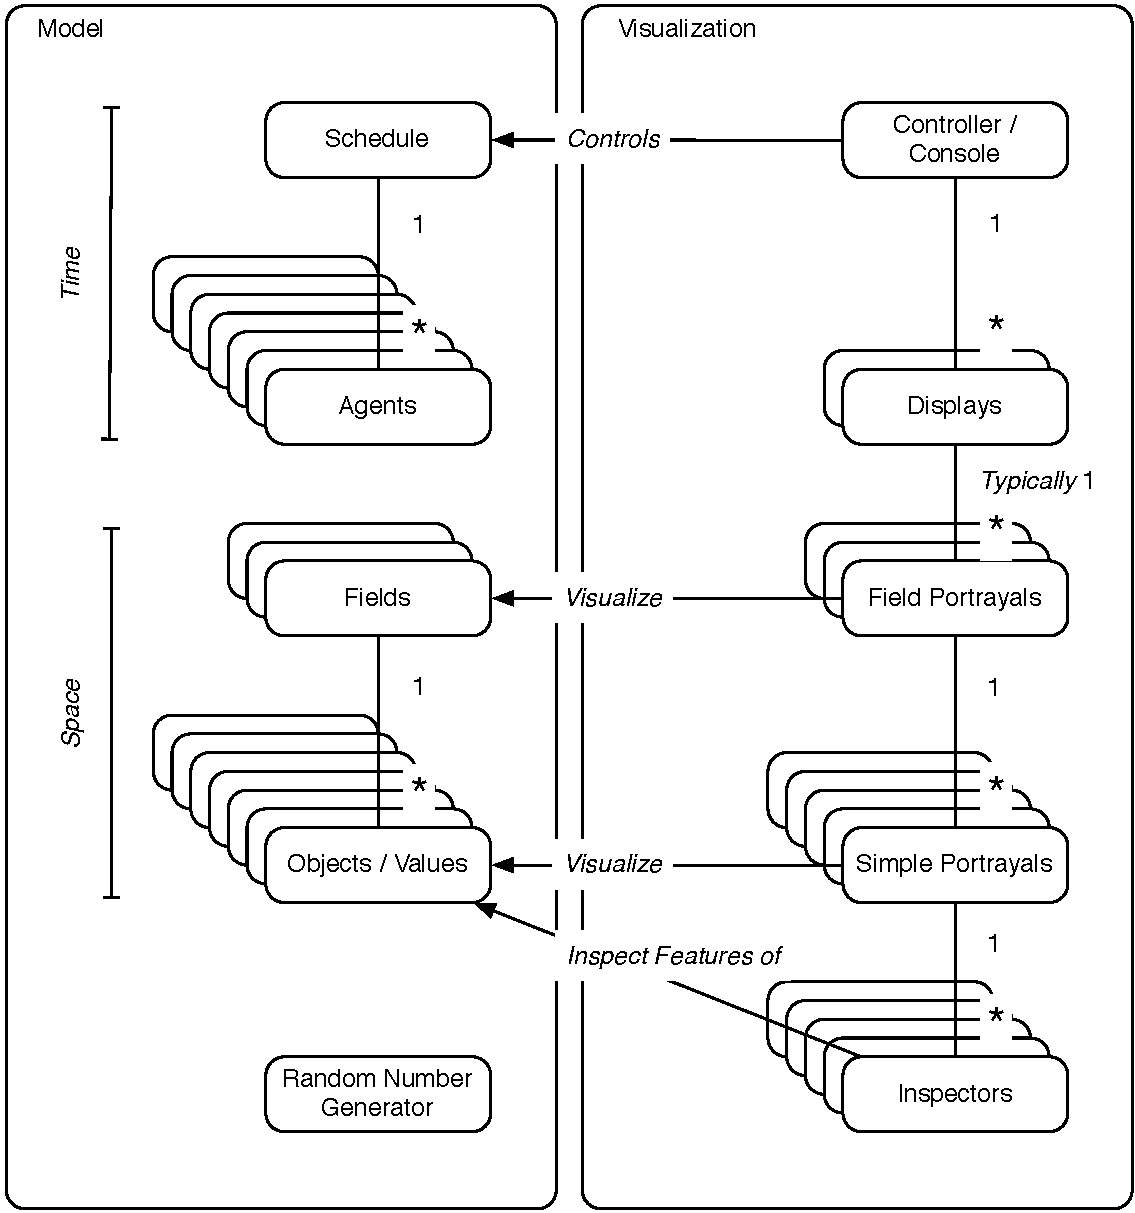
\includegraphics[width=3.7in]{MASONLayout.pdf}\vspace{-3em}\end{wrapfigure}

MASON is broken into two pieces.  The first part is the {\bf model} (the simulation proper) and the second part is the {\bf visualization}, presently either in 2D or in 3D.  Except when you choose to have model objects display themselves, the model and visualization are entirely separated.  This means that the model can be run without visualization; run with visualization of different sorts; and have its visualization changed, added, or removed at any time.  The model can also be {\bf checkpointed}, meaning it can be frozen and written out to disk, to be thawed out and continued even on another kind of computer.

At right is a general overview of the MASON architecture.

\paragraph{Model}  MASON's model is entirely encapsulated in a special object called \class{sim.engine.SimState}.  It contains a discrete event {\bf schedule} on which you can schedule various {\bf agents} to be called at some time in the future.  This facility is a MASON model's representation of {\bf time}. Additionally, the model contains one or more {\bf fields} to represent {\bf space}.  A field is nothing more than an arbitrary data structure relating various {\bf objects} or {\bf values} together.  MASON provides a number of built-in fields, such as networks, continuous space, and grids.  Last but not least, MASON's model contains a high-quality {\bf random number generator}.



\chapter{Reading and Writing Geospatial Data}
\label{ch:io}

This chapter covers recipes for reading and writing vector and grid based geospatial data.

\section{Reading Geospatial Data}
\label{sec:readingdata}
This section covers reading geospatial data into MASON using GeoMason.

\subsection{Reading a Shape File}
\label{sub:readingshapefiles}

\begin{description}
\item[Problem] ~\\
You want to read vector geospatial data stored in a Shape file.

\item[Solution]~\\
Create a \code{GeomVectorField} and use \code{ShapeFileImporter.read()} to load data into it.
\begin{Verbatim}[frame=lines,framesep=5mm,numbers=left,commandchars=+\[\]]
GeomVectorField vectorField = new GeomVectorField();

try {
   ShapeFileImporter.read("file:foo.shp", vectorField);
} catch (FileNotFoundException ex)
{  /* handle exception */  }
\end{Verbatim}

\end{description}

\paragraph{Discussion}



\subsection{Reading Multiple Vector Layers}
\label{sub:multiplevectorlayers}

\begin{description}
\item[Problem]~\\
You want to read in more than one thematic layer of vector data.

\item[Solution]~\\
After ensuring that each layer uses the same coordinate reference
system, read in each layer, and then synchronize the minimum bounding
rectangles for all the layers.
\begin{Verbatim}[frame=lines,framesep=5mm,numbers=left,commandchars=+\[\]]
GeomVectorField firstVectorField = new GeomVectorField();
GeomVectorField secondVectorField = new GeomVectorField();
GeomVectorField thirdVectorField = new GeomVectorField();

try {
   ShapeFileImporter.read("file:foo.shp", firstVectorField);
   ShapeFileImporter.read("file:bar.shp", secondVectorField);
   ShapeFileImporter.read("file:baz.shp", thirdVectorField);
} catch (FileNotFoundException ex)
{  /* handle exception */  }

Envelope globalMBR = firstVectorField.getMBR();

globalMBR.expandToInclude(secondVectorField.getMBR());
globalMBR.expandToInclude(thirdVectorField.getMBR());

firstVectorField.setMBR(globalMBR);
secondVectorField.setMBR(globalMBR);
thirdVectorField.setMBR(globalMBR);
\end{Verbatim}

\item[Discussion ]
\end{description}



\subsection{Reading a Shape File and Some of Its Attributes}
\label{sub:readingshapefileattributes}

\begin{description}
\item[Problem]~\\
You want to read a Shape file and only some of its associated attributes.

\item[Solution]~\\
Read in a shape file as in section \ref{sub:readingshapefiles}, but specify the desired attributes.
\begin{Verbatim}[frame=lines,framesep=5mm,numbers=left,commandchars=+\[\]]
GeomVectorField vectorField = new GeomVectorField();

Bag desiredAttributes = new Bag();
desiredAttributes.add("NAME");
desiredAttributes.add("TYPE");

try {
   ShapeFileImporter.read("file:foo.shp", vectorField, desiredAttributes);
} catch (FileNotFoundException ex)
{  /* handle exception */  }
\end{Verbatim}

\item[Discussion ]
\end{description}






\subsection{Reading an ARC/Info ASCII Grid File}
\label{sub:readinggridfile}

\begin{description}
\item[Problem]~\\
You want to read an Arc/Info ASCII Grid file.

\item[Solution]~\\
Create a \code{GeomGridField} and an \code{InputStream} opened on the grid file, then use \code{ArcInfoASCGridImporter()} to load the data into the grid field from the open input stream.
\begin{Verbatim}[frame=lines,framesep=5mm,numbers=left,commandchars=+\[\]]
	GeomGridField gridField = new GeomGridField();
	
	InputStream inputStream = new FileInputStream("foo.asc");
	ArcInfoASCGridImporter.read(inputStream, GridDataType.INTEGER, gridField);
\end{Verbatim}

\item[Discussion ]
\end{description}


\subsection{Reading a Mix of Grid and Vector Data}
\label{sub:readingmixofdata}

\begin{description}
\item[Problem]~\\
You want to read in multiple layers that are a mix of vector and grid geospatial data.

\item[Solution]~\\
After ensuring that all the layers have the same coordinate reference system, read all the layers into GeomVectorField or GeomGridFields, as appropriate, and then synchronize their respective minimum bounding rectangles.
\begin{Verbatim}[frame=lines,framesep=5mm,numbers=left,commandchars=+\[\]]
GeomVectorField vectorField = new GeomVectorField();
GeomGridField gridField = new GeomGridField();

try {
   ShapeFileImporter.read("file:vector.shp", firstVectorField);

   InputStream inputStream = new FileInputStream("grid.asc");
   ArcInfoASCGridImporter.read(inputStream, GridDataType.INTEGER, gridField);
} catch (FileNotFoundException ex)
{  /* handle exception */  }

Envelope globalMBR = vectorField.getMBR();

globalMBR.expandToInclude(gridField.getMBR());

vectorField.setMBR(globalMBR);
gridField.setMBR(globalMBR);
\end{Verbatim}

\item[Discussion ]
\end{description}




\section{Writing Geospatial Data}
\label{sec:writingdata}

\subsection{Writing a Shape File}
\label{sub:writingshapefile}

\begin{description}
\item[Problem]~\\
You want to save a GeoMason vector field to a Shape file.

\item[Solution]~\\
Use \code{ShapeFileExporter.write()} to save the vector field to a Shape file.
\begin{verbatim}
ShapeFileExporter.write("foo", vectorField);
\end{verbatim}
\item[Discussion]
 foo
\end{description}

\subsection{Writing an ARC/Info ASCII Grid File}
\label{sub:writinggridfile}

\begin{description}
\item[Problem]~\\
You want to write GeoMason grid data to an ARC/Info ASCII Grid file.

\item[Solution]~\\
Create a \code{Writer} for the grid file and use \code{ArcInfoASCGridExporter.write()} to write the \code{GeomGridField}.
\begin{Verbatim}[frame=lines,framesep=5mm,numbers=left,commandchars=+\[\]]
try {
   BufferedWriter writer = new BufferedWriter( new FileWriter("foo.asc") );
   ArcInfoASCGridExporter.write(gridField, writer);
   writer.close();
} catch (IOException ex)  {
   /* handle exception */
}
\end{Verbatim}

\item[Discussion] 

\end{description}






%\begin{figure}[h]\vspace{-33em}\hspace{30em}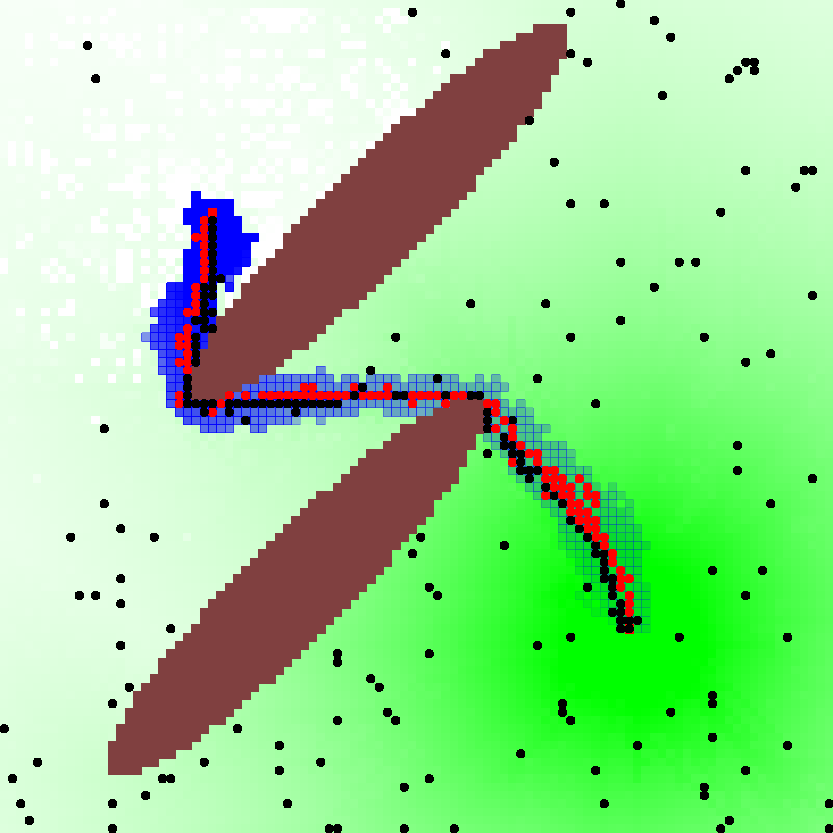
\includegraphics[width=4in]{ants.pdf}\vspace{2em}\end{figure}


%MASON has a large number of utility classes which can be used independently of the toolkit.  These classes fall in six packages:
%
%\begin{itemize}
%\item \package{ec.util}\quad The Mersenne Twister random number generator
%\item \package{sim.util}\quad Basic utility classes
%\item \package{sim.util.gui}\quad Graphical interface utility classes
%\item \package{sim.util.media}\quad Utility classes for generating various media (movies, pictures)
%\item \package{sim.util.media.chart}\quad Utility classes for generating charts
%\item \package{sim.util.distribution}\quad Utility classes for creating distributions
%\end{itemize} 
%
%This chapter concentrates solely on \package{ec.util}, \package{sim.util}, and \package{sim.util.distribution}.  Many classes in the core simulation code rely on these packages (well the first two anyway), so it's important to cover them. 
%
%\begin{methods}{\class{ec.util.MersenneTwisterFast}}
%\mthd{public void setSeed(long seed)} Seeds the random number generator.  Note that only the first 32 bits of the seed are used.
%\mthd{public void setSeed(int[] vals)} Seeds the random number generator using the given array.  Only the first 624 integers in the array are used.  If the array is shorter than 624, then the integers are repeatedly used in a wrap-around fashion (not recommended).  The integers can be anything, but you should avoid too many zeros.
%\mthd{public double nextDouble()} Returns a random double drawn in the half-open interval from [0.0, 1.0).  That is, 0.0 may be drawn but 1.0 will never be drawn.
%\mthd{public double nextDouble(boolean includeZero, boolean includeOne)} Returns a random double drawn in interval from 0.0 to 1.0, possibly including 0.0 or 1.0 or both, as specified in the arguments.
%\mthd{public float nextFloat()} Returns a random float drawn in the half-open interval from [0.0f, 1.0f).  That is, 0.0f may be drawn but 1.0f will never be drawn.
%\mthd{public float nextFloat(boolean includeZero, boolean includeOne)} Returns a random float drawn in interval from 0.0f to 1.0f, possibly including 0.0f or 1.0f or both, as specified in the arguments.
%\mthd{public double nextGaussian()} Returns a random double drawn from the standard normal Gaussian distribution (that is, a Gaussian distribution with a mean of 0 and a standard deviation of 1).
%\mthd{public long nextLong()} Returns a random long.
%\mthd{public long nextLong(long n)} Returns a random long drawn from between 0 to \(n-1\) inclusive.
%\mthd{public int nextInt()} Returns a random integer.
%\mthd{public int nextInt(int n)} Returns a random integer drawn from between 0 to \(n-1\) inclusive.
%\mthd{public short nextShort()} Returns a random short.
%\mthd{public char nextChar()} Returns a random character.
%\mthd{public byte nextByte()} Returns a random byte.
%\mthd{public void nextBytes(byte[] bytes)} Fills the given array with random bytes.
%\mthd{public boolean nextBoolean()} Returns a random boolean.
%\mthd{public boolean nextBoolean(float probability)} Returns a random boolean which is true with the given probability, else false.  Note that you must carefully pass in a {\it float} here, else it'll use the {\it double} version below (which is twice as slow).
%\mthd{public boolean nextBoolean(double probability)} Returns a random boolean which is true with the given probability, else false.
%\mthd{public Object clone()}  Clones the generator.
%\mthd{public boolean stateEquals(Object o)}  Returns true if the given Object is a MersenneTwisterFast and if its internal state is identical to this one.
%\mthd{public void writeState(DataOutputStream stream)}  Writes the state to a stream.
%\mthd{public void readState(DataInputStream stream)}  Reads the state from a stream as written by \method{writeState(...)}.
%\mthd{public static void main(String[] args)} Performs a test of the code.
%\end{methods}


\chapter{Displaying Geospatial Data}
\label{ch:displaying}

This chapter gives recipes for displaying GeoMason fields in MASON.

%\begin{figure}[h]\vspace{-26em}\hspace{25.3em}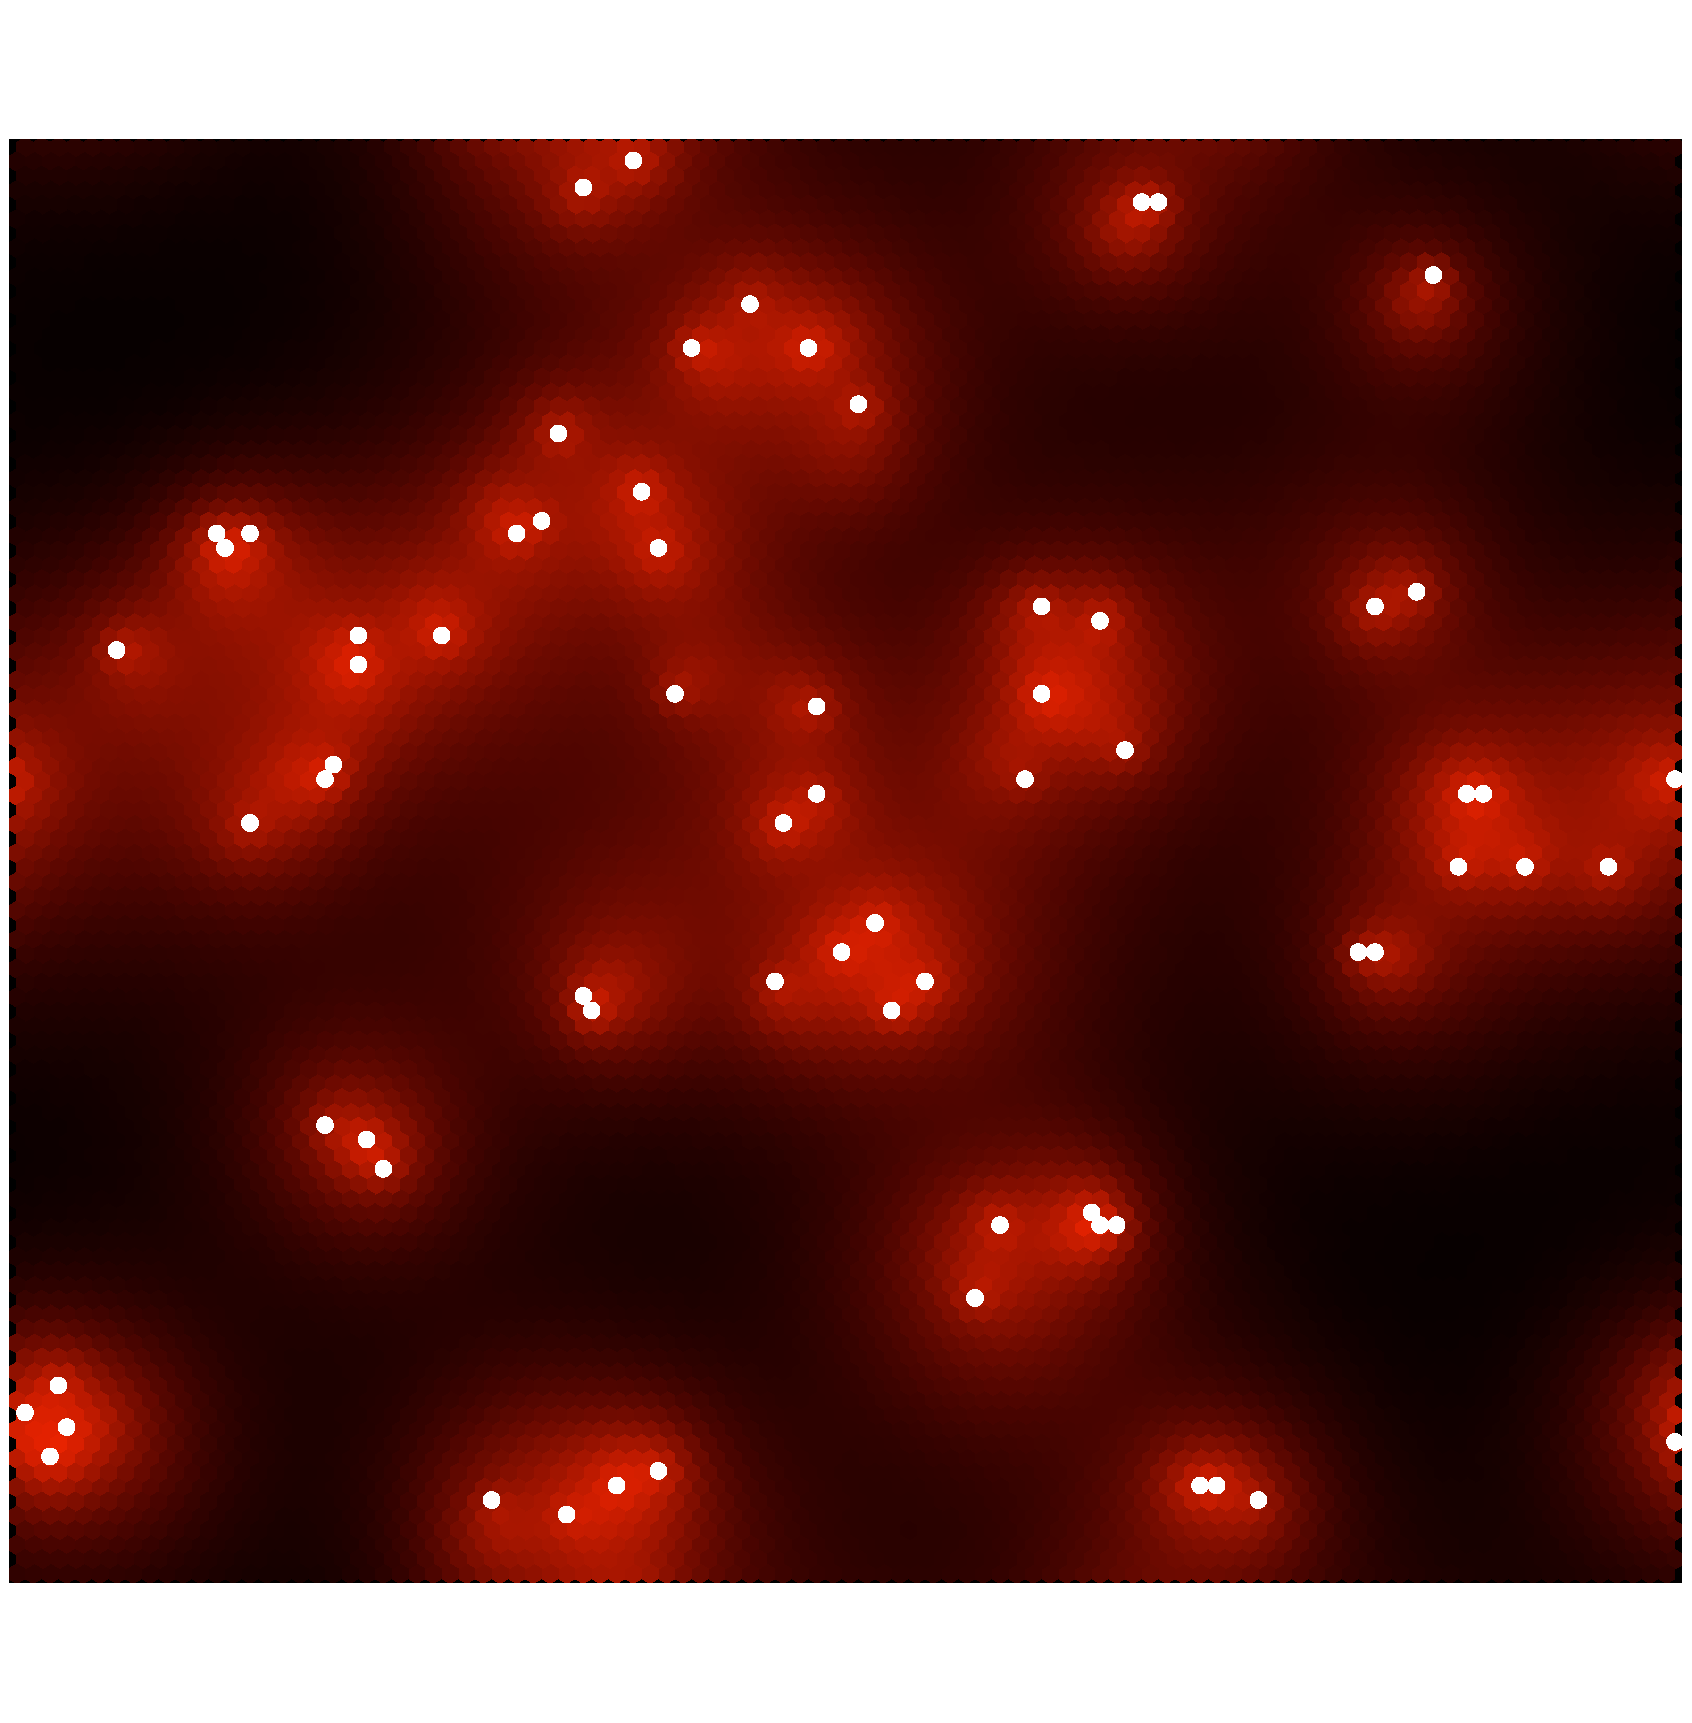
\includegraphics[width=4in]{hexabugs.pdf}\vspace{2em}\end{figure}

%\noindent A {\bf grid} is MASON's name for objects arrange in a 2-dimensional or 3-dimensional array or equivalent.  MASON supports a wide range of grid environments as fields (representations of space).  This includes most any combination of the following:

\section{Displaying a \code{GeomVectorField}}
\label{sub:displayingGeomVectorField}

\begin{description}
\item[Problem]~\\
You want to show the contents of a \code{GeomVectorField} in a
MASON display.

\item[Solution]~\\
Create a \code{GeomVectorFieldPortrayal} in the MASON \code{GUIState}
subclass, associate it with its corresponding \code{GeomVectorField},
set up an appropriate MASON or GeoMason field portrayal, and attach it
to a MASON \code{Display2D} object.

\begin{Verbatim}[frame=lines,framesep=5mm,numbers=left,commandchars=+\[\]]
public class MyMasonGUI extends GUIState
{
    private Display2D display;
    private JFrame displayFrame;

    // ... other variable declarations

    +color[red]private GeomVectorFieldPortrayal myPortrayal = new GeomVectorFieldPortrayal();

    @Override
    public void init(Controller controller)
    {
        super.init(controller);

        display = new Display2D(ARBITRARY_WIDTH, ARBITRARY_HEIGHT, this);

        +color[red]display.attach(myPortrayal, "My Vector Layer");

        displayFrame = display.createFrame();
        controller.registerFrame(displayFrame);
        displayFrame.setVisible(true);
    }

    @Override
    public void start()
    {
        super.start();
        setupPortrayals();
    }

    private void setupPortrayals()
    {
        MyState world = (MyState)state;

        +color[red]myPortrayal.setField(world.vectorLayer);
        +color[red]myPortrayal.setPortrayalForAll(new GeomPortrayal(Color.CYAN, true));+label[ex:trueforfill]

        display.reset();
        display.setBackdrop(Color.WHITE);

        display.repaint();
    }

    // ... other code
}
\end{Verbatim}

\item[Discussion ]~\\

Line \ref{ex:trueforfill} creates a portrayal that draws all the lines
in cyan; the optional second parameter, which is set to \code{true}, indicates
that polygons should be filled.
\end{description}





\section{Displaying a \code{GeomGridField}}
\label{sec:displayinggridfield}

\begin{description}
\item[Problem]~\\
You want to show the contents of a \code{GeomGridField} in a MASON display

\item[Solution]~\\
Problem Solution
\begin{Verbatim}[frame=lines,framesep=5mm,numbers=left,commandchars=+\[\]]
\end{Verbatim}

\item[Discussion ]
\end{description}



\section{Displaying a Boundary Over a Grid Field}
\label{sec:boundaryovergrid}

\begin{description}
\item[Problem]~\\
You want to overlay political boundaries on grid data.

\item[Solution]~\\
Problem Solution

\begin{Verbatim}[frame=lines,framesep=5mm,numbers=left,commandchars=+\[\]]
\end{Verbatim}

\item[Discussion ]
\end{description}



\chapter{Common Problems}
\label{ch:commonprobs}


\section{Display All One Color}
\label{sec:OneColorDisplay}

\begin{description}
\item[Problem]~\\
Rendering a \code{GeomField} just shows one solid color.

\item[Solution]~\\
Problem Solution
\begin{Verbatim}[frame=lines,framesep=5mm,numbers=left,commandchars=+\[\]]
\end{Verbatim}

\item[Discussion ]
\end{description}


\section{Layers Do Not Align}
\label{sec:NonAlignedLayers}

\begin{description}
\item[Problem]~\\
The data between layers does not match.

\item[Solution]~\\
Problem Solution
\begin{Verbatim}[frame=lines,framesep=5mm,numbers=left,commandchars=+\[\]]
\end{Verbatim}

\item[Discussion ]
\end{description}





\cleardoublepage
\footnotesize
\addcontentsline{toc}{chapter}{Index}
\printindex

\end{document}















